\newpage
\section{Architettura}

\subsection{Pattern Architetturale}
Il pattern architetturale scelto per questo progetto è il celebre \textbf{MVC}.
Questa scelta ha portato ad una divisione netta dei compiti tra i vari componenti. In fase di design il pattern si
è rivelato importante perchè ci ha permesso di dividere in maniera ottimale il flusso di lavoro e i task che ognuno dei
componenti doveva portare a termine. Questa scelta, unita al \textit{modello ad attori}, ha aiutato
lo sviluppo permettendoci di astrarre alcuni concetti e rendere il più indipendenti possibili i vari componenti del software.

\subsection{Modello ad Attori}
La presenza di un elevato numero di entità all’interno dell’applicazione ha portato alla luce
l’esigenza di gestire, già a livello architetturale, la possibilità di sfruttare a pieno la potenza
della cpu, rendendo quindi il programma concorrente. \\
In particolare, per astrarre dalla gestione
di problematiche tipiche di sistemi concorrenti (mutua eclusione e corse critiche) si è deciso di
adottare un approccio basato su attori.\\
Dal momento che ogni attore incapsula al suo interno
un flusso di controllo basato su \textit{event loop} e che le interazioni avvengono esclusivamente
attraverso scambio di messaggi, non è necessario gestire meccanismi di sincronizzazione. \\
Inoltre, abbiamo ritenuto il modello ad attori particolarmente adeguato per la realizzazione
dell’applicazione in quanto essi incapsulano il \textbf{comportamento}, delle entità all’interno del modello. \\
Per tali motivi si è deciso quindi di adottare il framework
\textit{Akka} per sviluppare in maniera semplificata il sistema ad attori.

\subsubsection{Vantaggi del Modello ad Attori}
Di seguito si analizzano i vantaggi dell'utilizzo di Akka:
\begin{itemize}
    \item Chiarezza del comportamento del sistema fin da subito.
    \item Espressività del codice relativo al comportamento delle entità di gioco.
    \item Migliore incapsulamento dei task di ogni componente.
    \item Sistema maggiormente modulare.
    \item Astrazione di meccanismi di concorrenza di basso livello (semafori, monitor, ecc.).
\end{itemize}

\subsubsection{Svantaggi del Modello ad Attori}
Alcune criticità dell'utilizzo di Akka sono le seguenti:
\begin{itemize}
    \item Difficoltà nel testing degli attori.
    \item Il numero dei messagi scambiati è proporzionale alla dimensione del sistema.
    \item Eventuale \textit{bottleneck} dovuto al message passing.
\end{itemize}

\subsection{Architettura Complessiva}
L'impiego del paradigma ad attori combinato al pattern architetturale MVC ci ha portato a modellare questi tre componenti
come essi stessi attori. Ognuno di essi gestisce messaggi di tipo diverso:
\begin{itemize}
    \item \textit{Command} - questo è il tipo di messaggio accettato dal GameLoop ovvero l'attore che fungerà da
    Controller del sistema. Questa tipologia di messaggi indica tutte le interazioni tra Controller, Model e View.
    \item \textit{ModelMessage} - questo è il tipo di messaggio accettato dagli attori del Model. I messaggi di questa categoria
    gestiranno l'avanzamento dello stato interno degli oggetti di Model.
    \item \textit{ViewMessage} - questo è il tipo di messaggio accettato dal ViewActor ovvero l'attore che fungerà da View
    del sistema. Questa serie di messaggi delineerà l'API per le interazioni tra View, Controller e utente finale.
\end{itemize}

\begin{figure}[H]
    \centering
    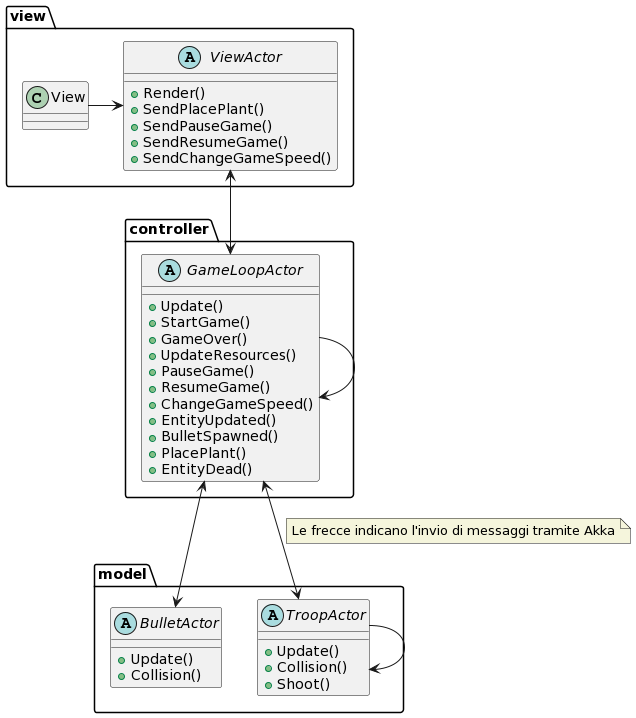
\includegraphics[width=\linewidth]{images/actor-architecture}
    \label{Diagramma delle classi dell'architettura complessiva.}
    \caption{Architettura finale dell'actor system.}
\end{figure}

È stato utilizzato il formalismo UML per modellare gli attori,
tuttavia, sono state adottate alcune convenzioni per facilitarne la compresione.
Le frecce rappresentato le interazione ad alto livello che avvengono tra i vari componenti.
Nonostante l'immagine  suggerisca la violazione del pattern MVC, le frecce rappresentano in realtà il flusso dei messaggi.
Per fare un esempio, gli attori del Model non inizieranno mai una relazione con il Controller,
bensì si limitano a rispondere ai messaggi che quest'ultimo spedisce.